\section{Ground Station localization}
The place where the Ground Stations would be placed has to be studied in order to obtain maximum rendiment of them. This decision will depend mainly of the constellation characteristics, the earth topography and the country legislation and resources. In this chapter the analysis and procedures for arriving to the final decision of where the Ground Stations would be placed are exposed.\\
Given the constellation topology, the coverage of a Ground Station depending on its longitude and latitudecwill be studied. The aim of this analysis is to show where a Ground Station would have more coverage and give a first approximation and proposal of the 3 Ground Station placement.
\subsection{Method}
For the purpose above explained, a Matlab algorithm is developed. This algorithm calculates, on a given moment, how many satellites can be seen from a Ground Station. This calculation will be done several times in order to obtain results along time. In order to elaborate the algorithm the steps showed below are followed:
\begin{enumerate}
\item Calculate where the satellites are refereed to an inertial Cartesian coordinates system, with the origin at the center of the Earth. This state analysis is done for several time periods with an adequate time-step. 
\item Calculate the Ground Station position refereed to the mentioned system. Since the system is inertial, the Ground Station will describe a circle in the rotational plane of the Earth relative to this system. This trajectory depend on the latitude and longitude of the place. This position is calculated for the same time period used before.
\item Calculate, for each time step, how many links can the GS establish. It will depend on the angle between the station and every satellite, and also on the minimum elevation angle. 
\end{enumerate}
After seeing reasonable results modifying the parameters of the constellation and of the Ground station, the algorithm will be verified simulating the Iridium constellation. Entering the parameters of this system, the results verifies the algorithm.\\
Once the algorithm is tested and verified, the links during the day for several longitudes and latitudes and how this parameters affect to the coverage of the station are studied\footnote{The code can be found at the annexes.}
\subsection{Latitude analysis}
Is easy to see that the effect of changing the latitude is practically independent for the longitude. For this reason, the links during the day for a given longitude are studied independently of the latitude and viceversa. Doing the analysis for latitudes between 0º and 90º during 2 days, with 5 minutes time-step, this are the results:

\begin{figure}[H]
\begin{center}
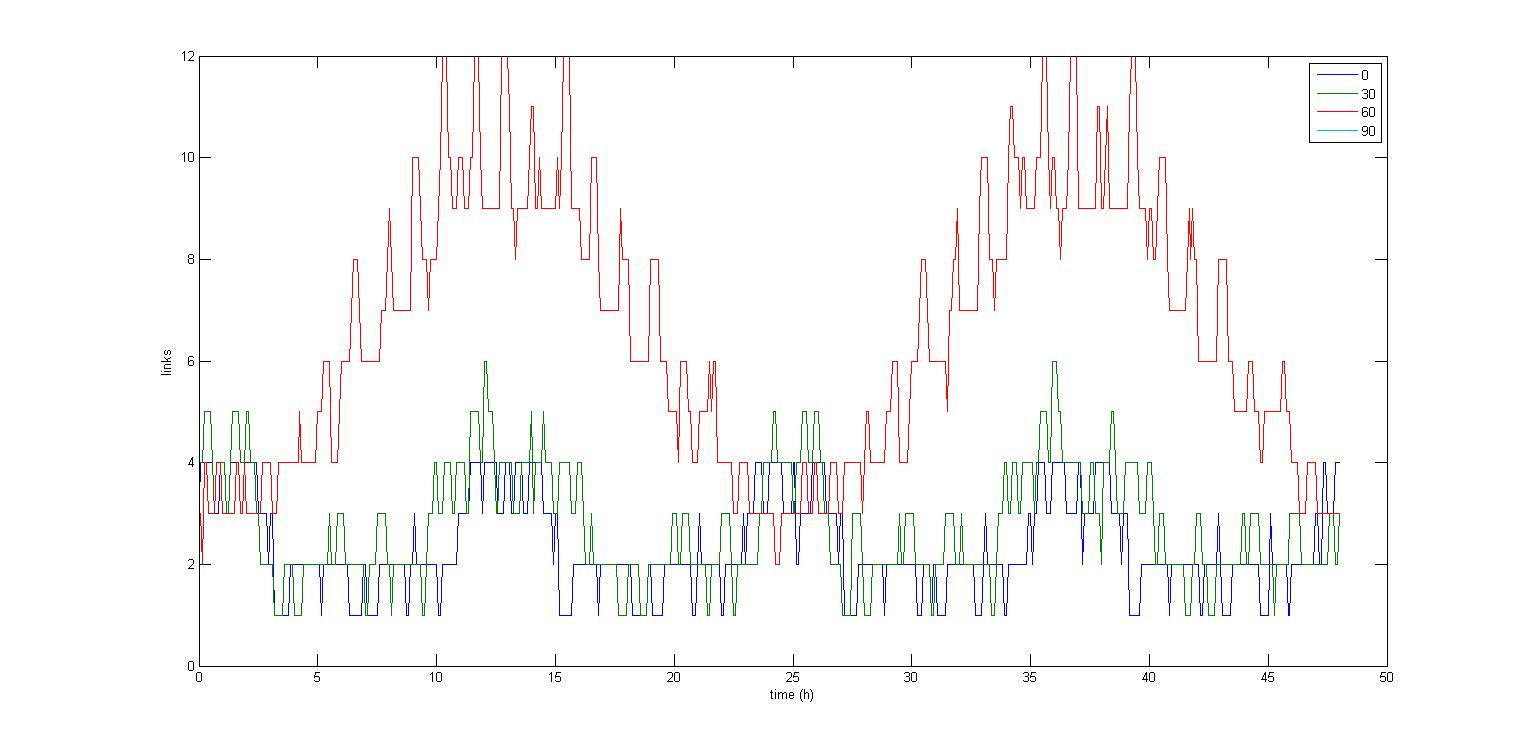
\includegraphics[scale=0.30]{0_30_90_lat.jpg}
\caption{Links vs time for latitudes from 0º to 90º}
\end{center}
\end{figure}
As is shown in Figure 1.1, the behaviour is not constant during the day. For every day there is a peak and a valley. This is produced for the cylindrical asymmetry of the constellation. It can also be seen that the pole is not covered. This fact was considered and assumed at the design of the constellation since it doesn't involve any problem at the performance of the system. It can also be seen that for an equatorial latitude there is always 1 link, at least. The equator is the most critical place because is where satellites from different planes are more separated. Global coverage can be ensured, but is important to appreciate that for higher latitudes the coverage is better.\\
Doing the same analysis but for negative latitudes, the following results are obtained:
\begin{figure}[H]
\begin{center}
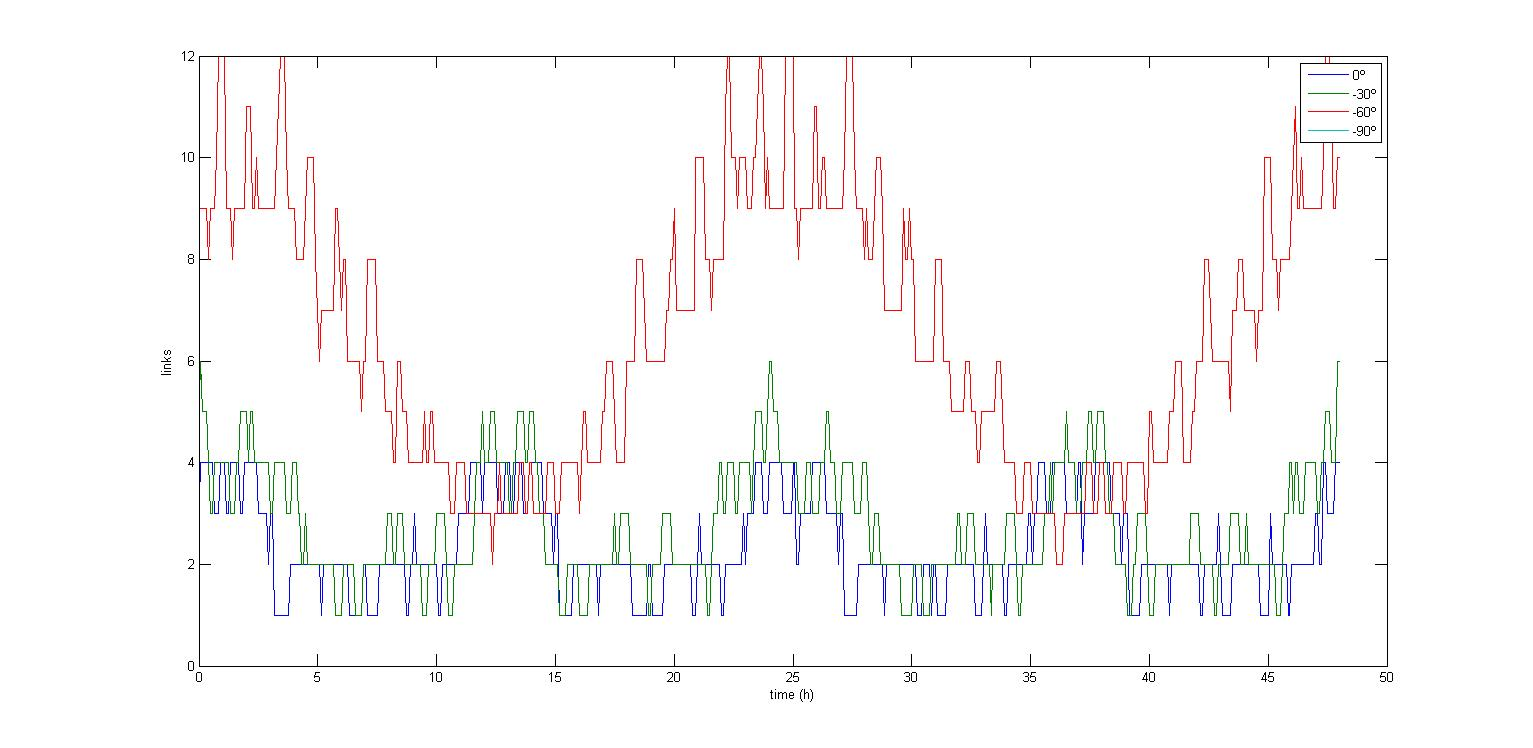
\includegraphics[scale=0.30]{0_-30_-90_lat.jpg}
\caption{Links vs time for latitudes from 0º to -90º}
\end{center}
\end{figure}
Comparing the results of Figure 1.2 with the ones of Figure 1.1 it is seen that they are practically the same but with an offset of 12 hours. They are also seen small local deviations, but these are not much significant because of the time-step. This time-step is of 5 minutes for a first sight of the tendencies, and it do not allow extremely precise results.\\
Taking into account that the results of positive latitudes can be extrapolated to negative ones, the rest of the analysis will be done only for positive latitudes.Is important to know at which latitude, close to the poles, the coverage is lost due to the geometry of the constellation.
\begin{figure}[H]
\begin{center}
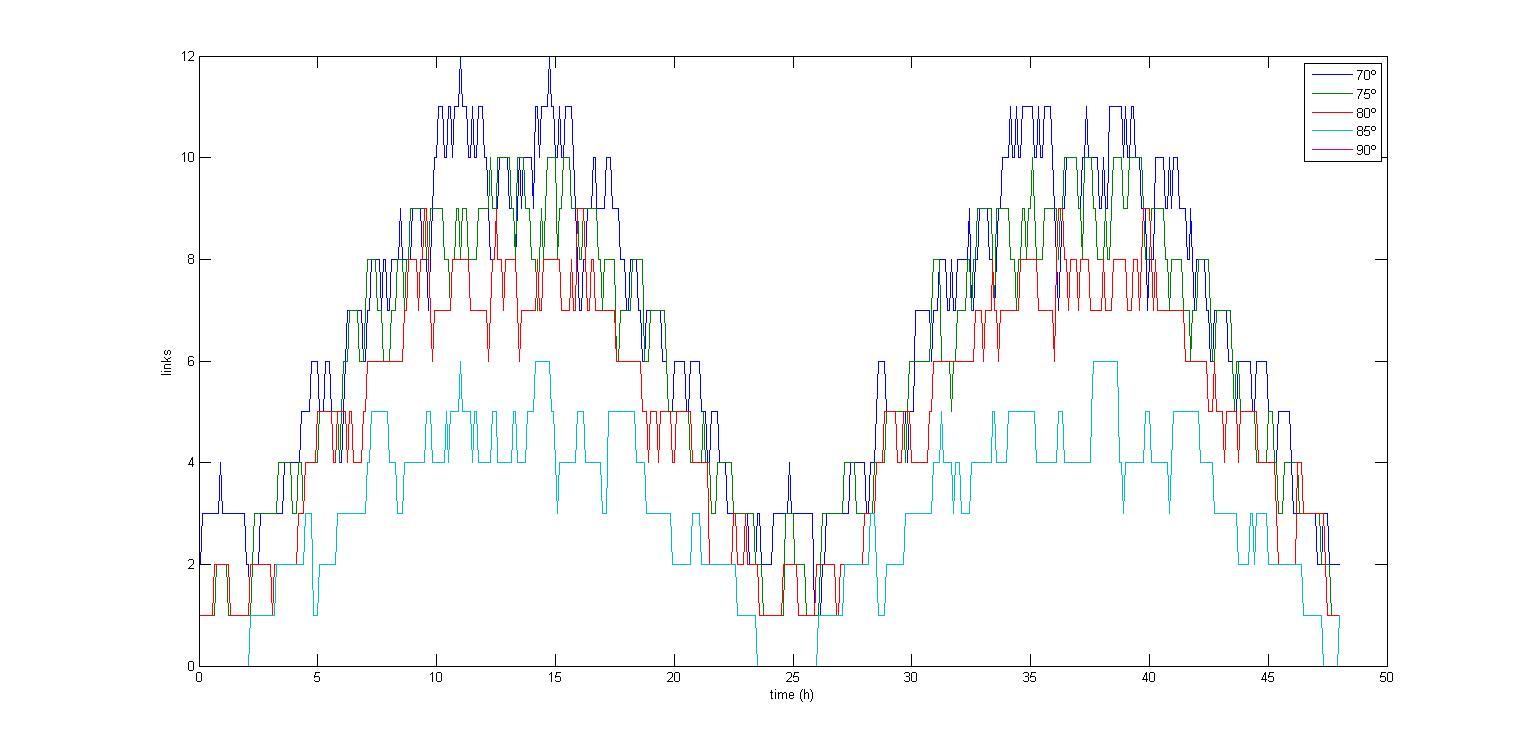
\includegraphics[scale=0.30]{70_5_90_lat.jpg}
\caption{Links vs time for latitudes from 70º to 90º}
\end{center}
\end{figure}
It is seen that over 80º of latitude the system starts to lose coverage. It does not cause any problem because there are not inhabited zones over +80º or under -80º. For situating the Ground Stations it has to be considered this restriction.\\
Now, the latitudes that can provide more links are, around 60º:
\begin{figure}[H]
\begin{center}
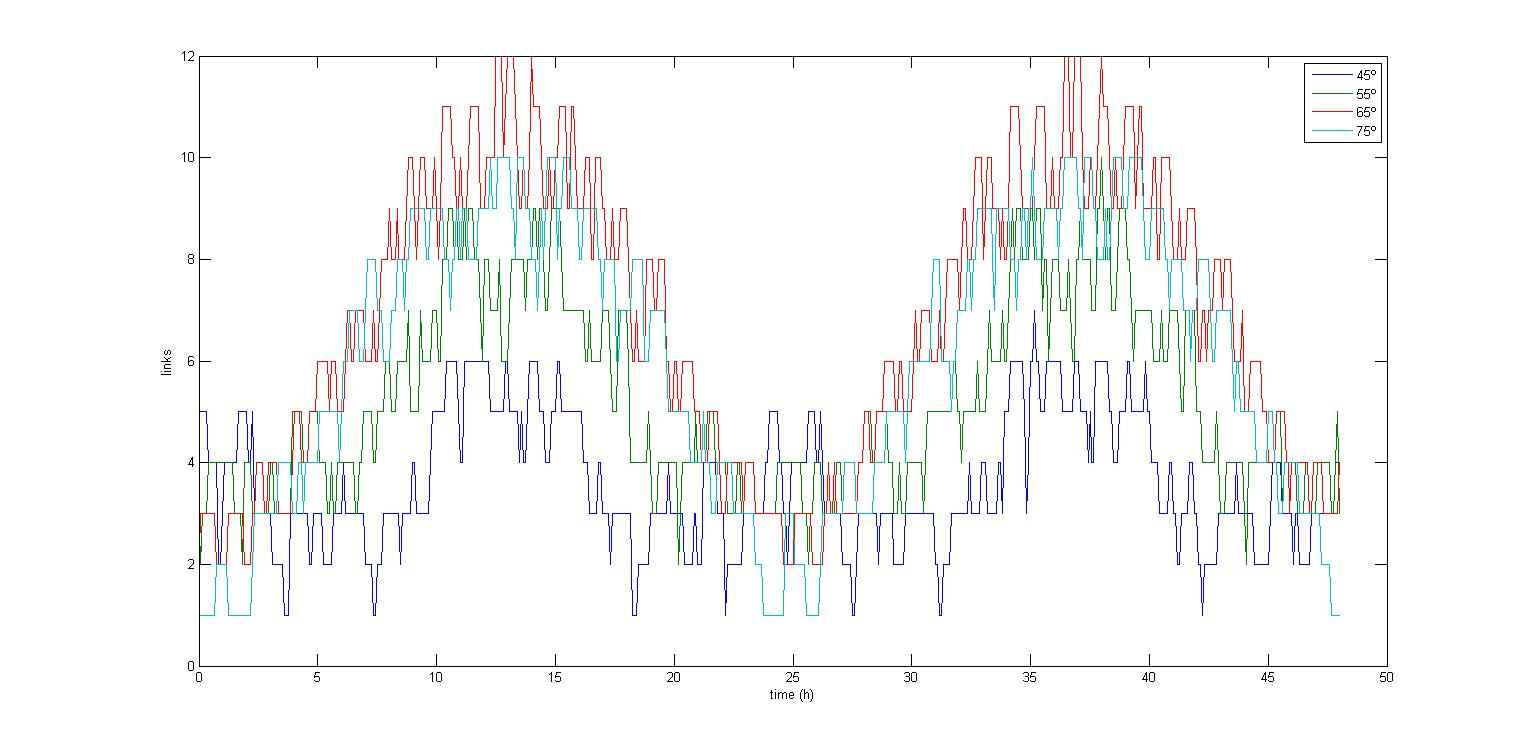
\includegraphics[scale=0.30]{45_10_75_lat.jpg}
\caption{Links vs time for latitudes from 45º to 75º}
\end{center}
\end{figure}
As it can be seen in Figure 1.4, the optimal latitude must be between 55º and 75º. Expanding the analysis:
\begin{figure}[H]
\begin{center}
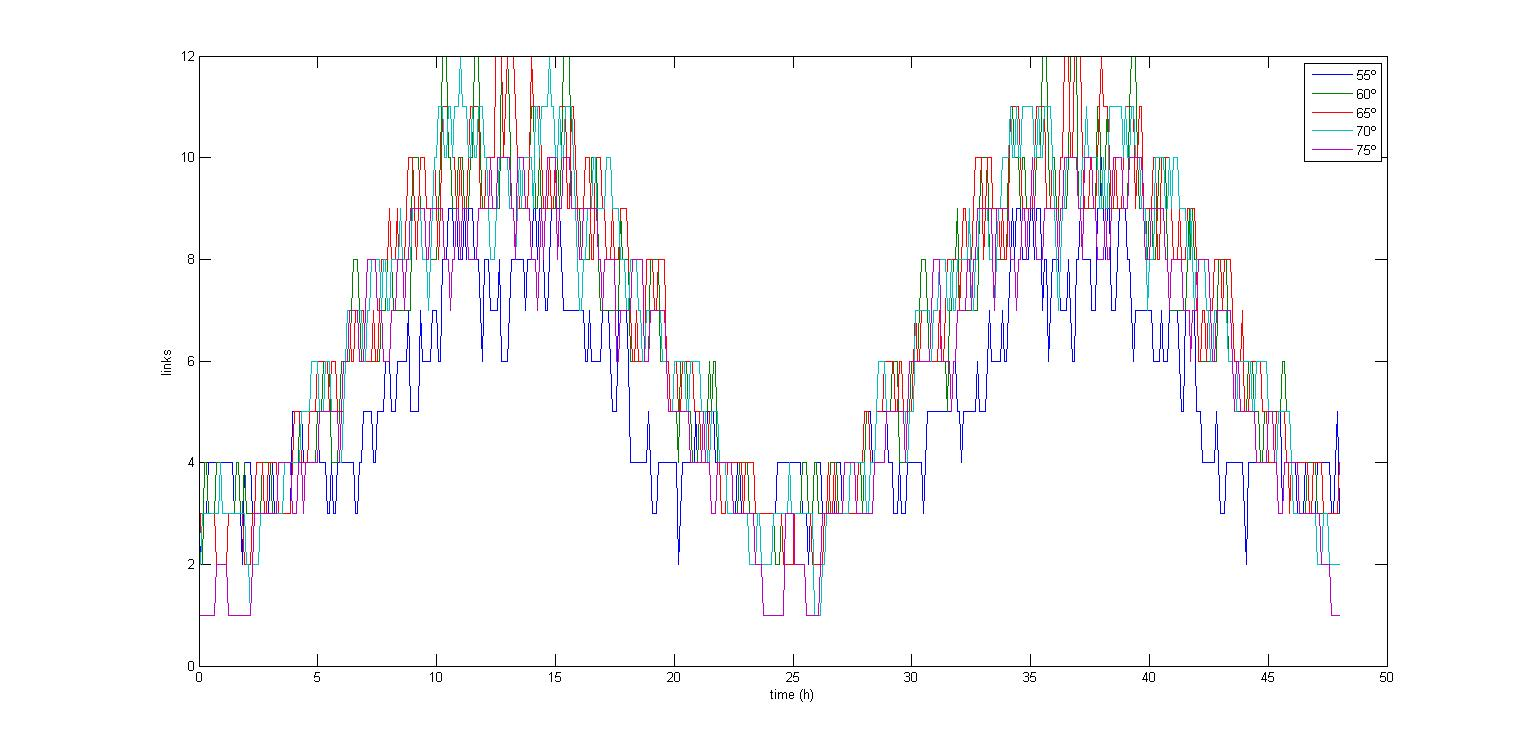
\includegraphics[scale=0.30]{55_5_75_lat.jpg}
\caption{Links vs time for latitudes from 55º to 75º}
\end{center}
\end{figure}
The better performance is registered around 60º and 65º. Figure 1.5 suggest that between 50º and 60º there is always at least 1 link. But looking it carefully, at the hour 37, there is a local deviation to 0 links. This requires a more accurate analysis decreasing the time-step. For 30 seconds time-step:
\begin{figure}[H]
\begin{center}
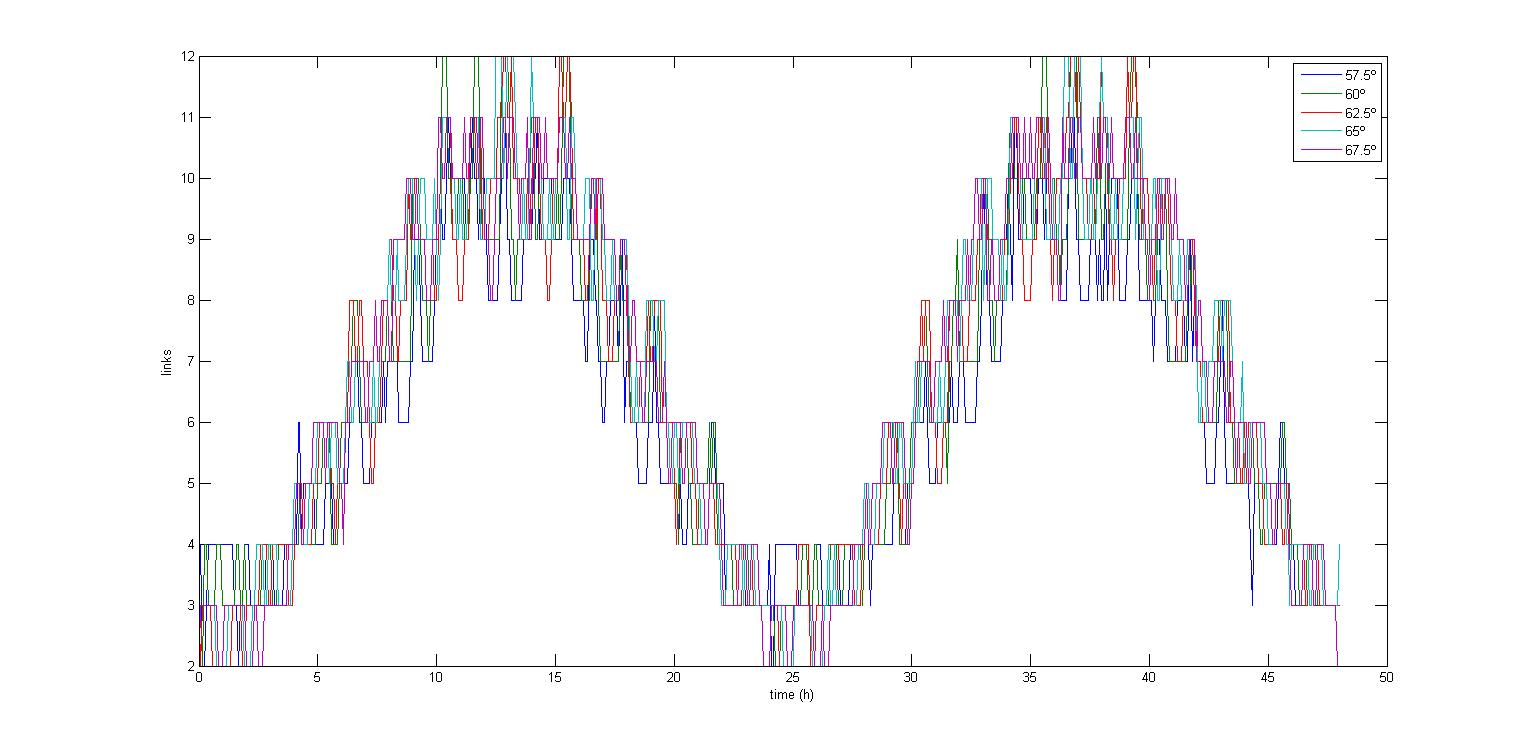
\includegraphics[scale=0.30]{575_25_675_lat.jpg}
\caption{Links vs time for latitudes from 57.5º to 67.5º}
\end{center}
\end{figure}
In Figure 1.6 there is no problem with the coverage. For ensuring the results and to avoid possible loses of links locally in time, the same ragne of latitudes is analyze with a smaller time-step.
\begin{figure}[H]
\begin{center}
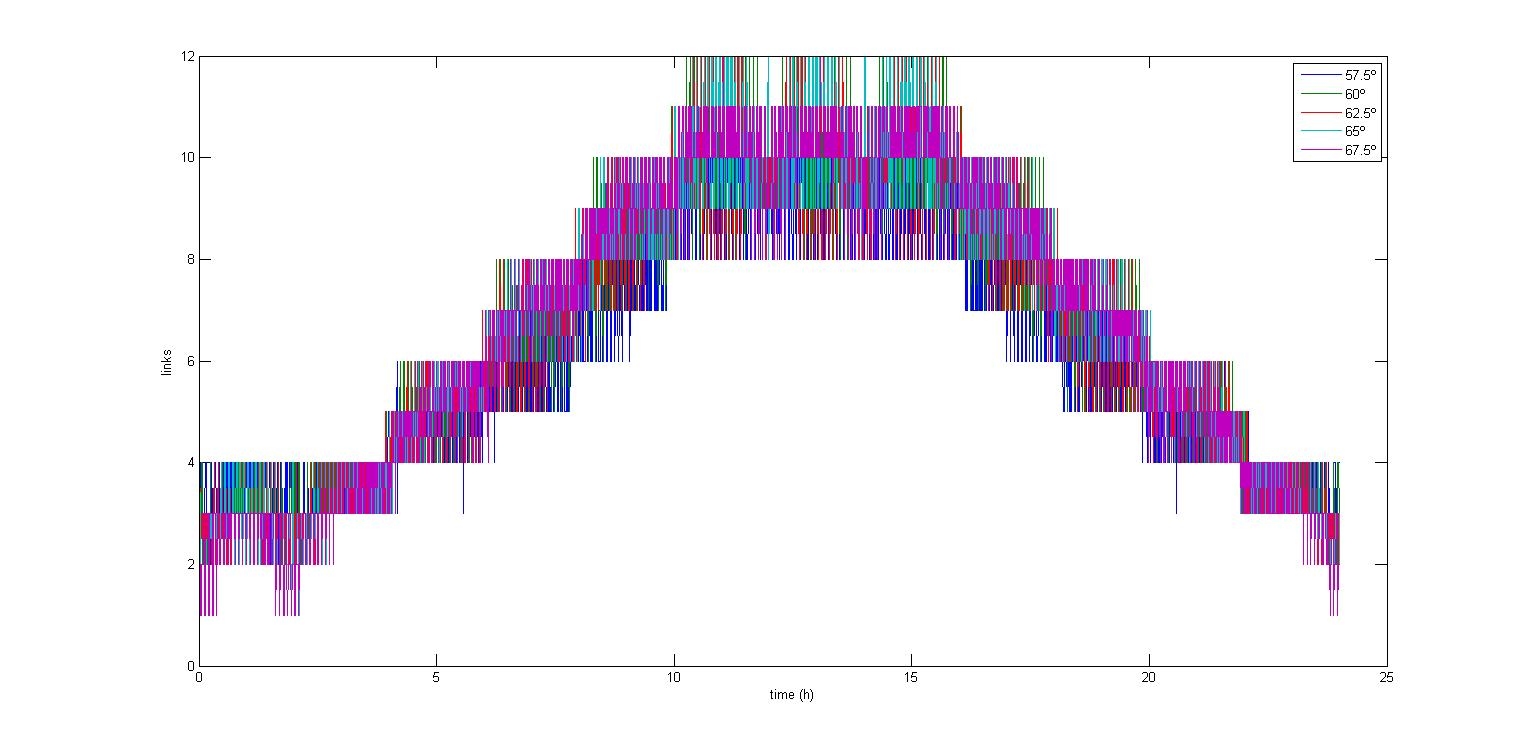
\includegraphics[scale=0.30]{575_25_675_(30s)_lat.jpg}
\caption{Links vs time for latitudes from 57.5º to 67.5º with 30 seconds time-step}
\end{center}
\end{figure}
It can be seen that between 65º and 67.5º the system loses the 2nd link and for a wile the station would be connected only to 1 satellite. It is optimum to place the stations between +57.5º and +62.5º of latitude. In order to verify the results for the opposite latitudes:
\begin{figure}[H]
\begin{center}
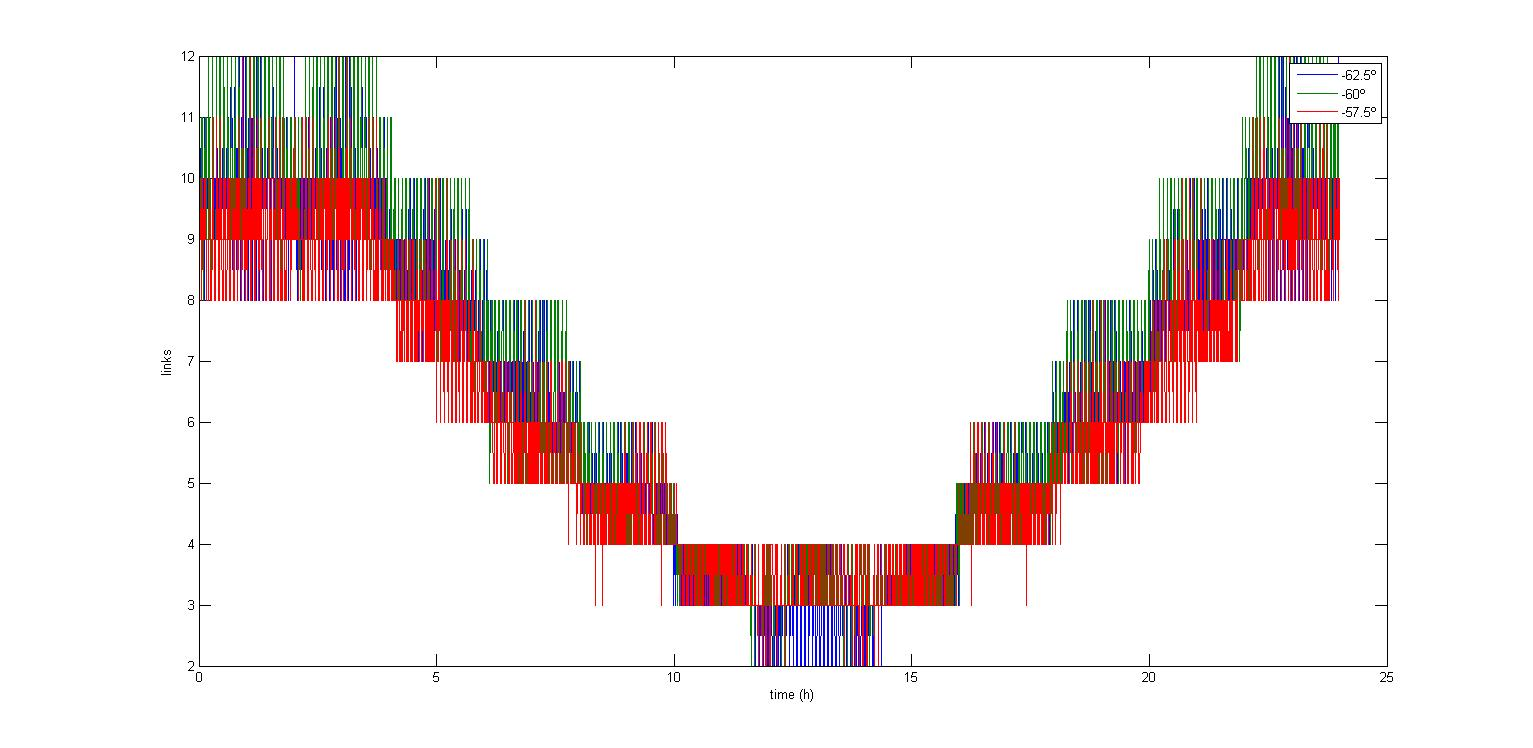
\includegraphics[scale=0.30]{-625_-25_575_(30s)_lat.jpg}
\caption{Links vs time for latitudes from -62.5º to -57.5º with 30 seconds time-step}
\end{center}
\end{figure}
In conclusion, the optimum latitudes for the Ground Station are:
\begin{itemize}
\item Between -62.5º and -57.5º
\item Between +57.5º and +62.5º
\end{itemize}

\subsection{Longitude analysis}
It is intuitive to think that the effect of changing the longitude is delaying the evolution of the coverage. This effect is verified by the algorithm:

\begin{figure}[H]
\begin{center}
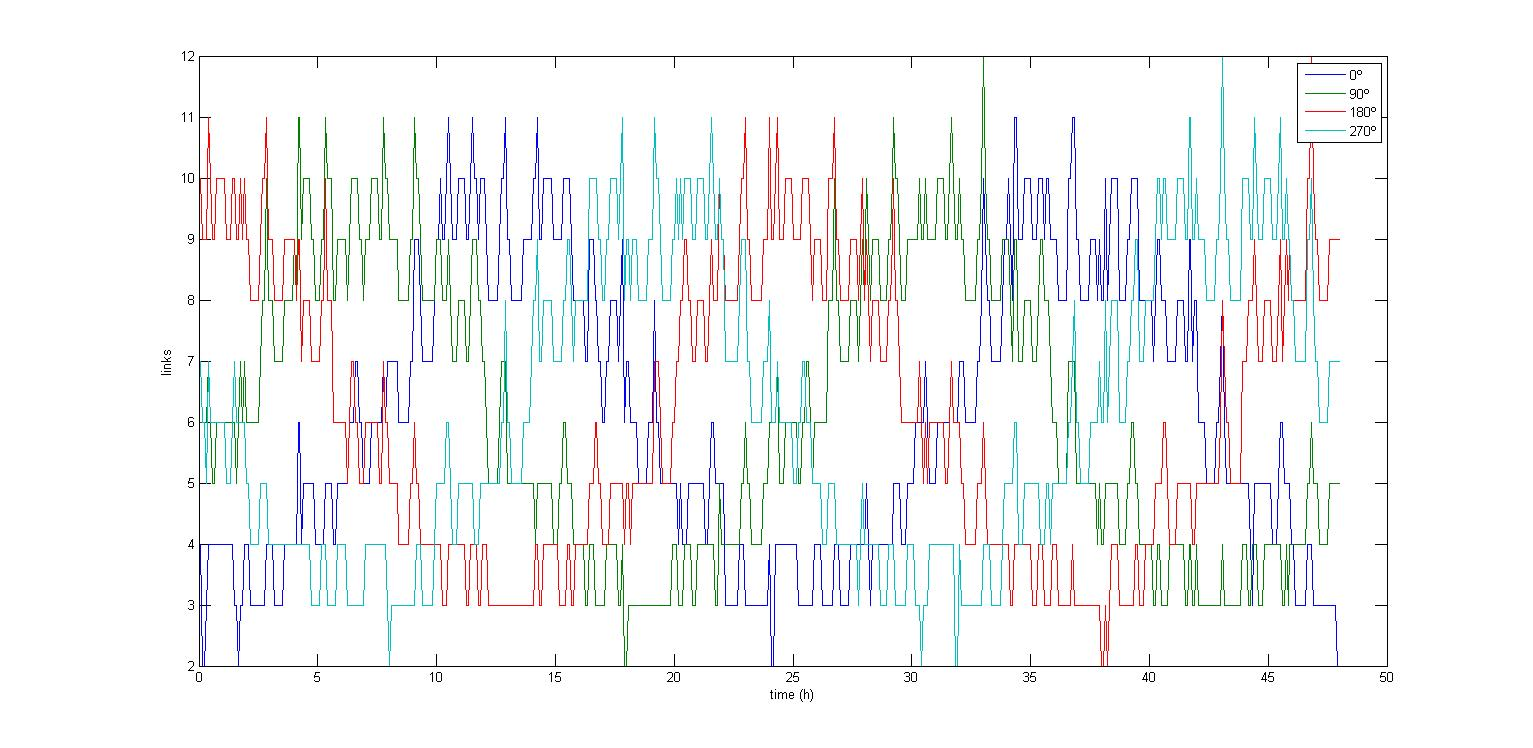
\includegraphics[scale=0.30]{0_90_270_long.jpg}
\caption{Links vs time for longitudes from 0º to 270º}
\end{center}
\end{figure}


As it is seen in Figure 1.8 the delay has a reason of 3 hours for every 45º of longitude. This effect can be used in order to optimize the performance of the Ground Stations. During the day every station will have a peak and a valley in the coverage. Placing the stations with a relative longitude of 120º would ensure that when one is at the valley another one is at the peak:

\begin{figure}[H]
\begin{center}
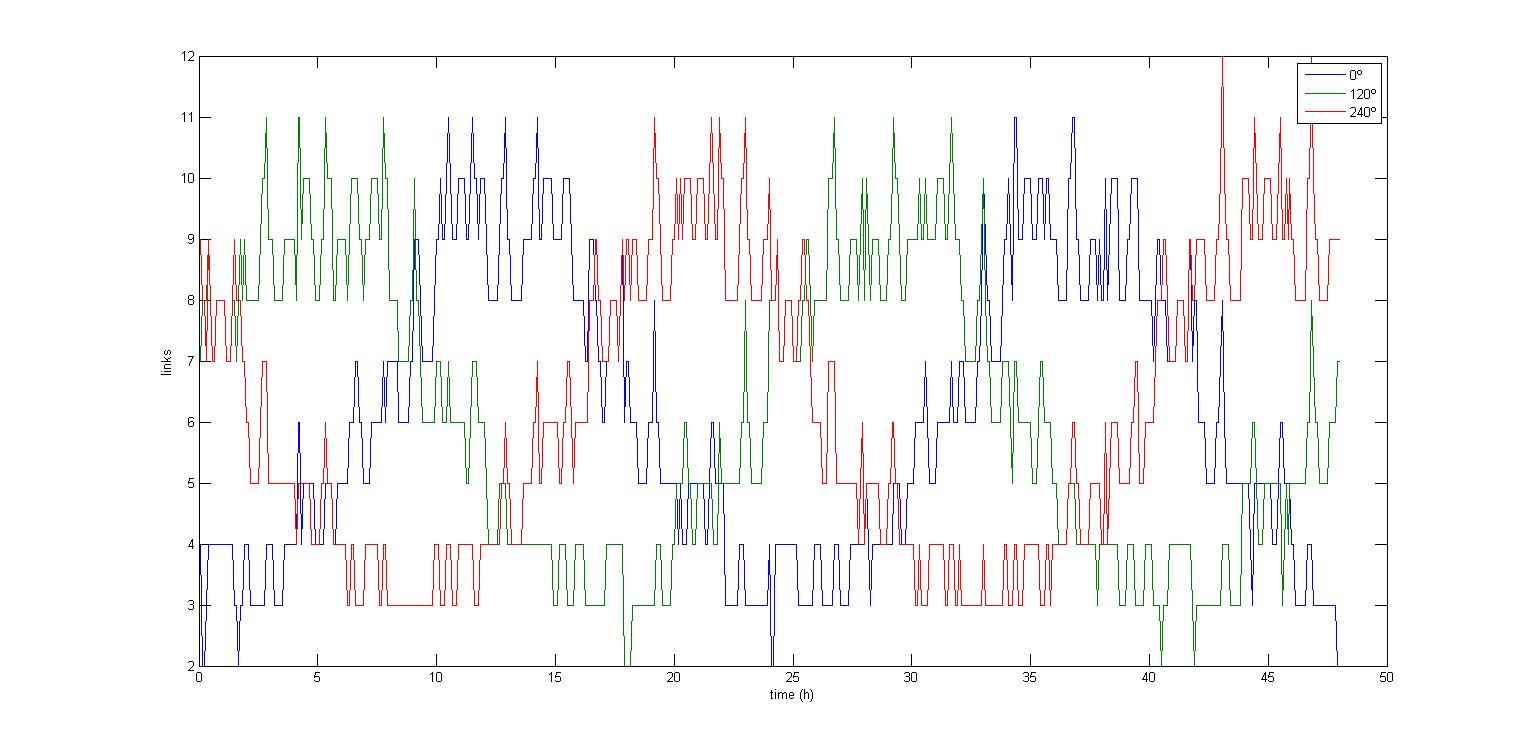
\includegraphics[scale=0.30]{0_120_240_long.jpg}
\caption{Links vs time for longitudes of 0º, 120º and 240º}
\end{center}
\end{figure}
In conclusion, the Ground Stations should be separated 120º longitude between them. It has to be taken into account that this analysis is done for stations at the same latitude. A Ground Station in a given latitude has the same coverage behaviour as an other one at the opposite latitude and 180º of longitude away. To exemplify, in the following table coordinates of equivalent places from the Ground Station point of view are showed. 
\begin{table}[H]
\begin{center}
\begin{tabular}{|c|c|c|c|c|c|c|}
\hline 
 & \multicolumn{2}{c|}{GS1} & \multicolumn{2}{c|}{GS2} & \multicolumn{2}{c|}{GS3} \\ 
\hline 
 & Latitude & Longitude & Latitude & Longitude & Latitude & Longitude \\ 
\hline 
Option 1 & 55 & 0 & 55 & 120 & 55 & 240 \\ 
\hline 
Option 2 & -55 & 180 & 55 & 120 & 55 & 240 \\ 
\hline 
Option 3 & 55 & 0 & -55 & 300 & 55 & 240 \\ 
\hline 
Option 4 & 55 & 0 & 55 & 120 & -55 & 60 \\ 
\hline 
Option 5 & -55 & 180 & -55 & 300 & 55 & 240 \\ 
\hline 
Option 6 & -55 & 180 & 55 & 120 & -55 & 60 \\ 
\hline 
Option 7 & 55 & 0 & -55 & 300 & -55 & 60 \\ 
\hline 
Option 8 & -55 & 180 & -55 & 300 & -55 & 60 \\ 
\hline 
\end{tabular}
\caption{Equivalent coordenates}
\end{center}
\end{table}
\subsection{Conclusion}
Summarizing the results of the analysis, for an optimum performance of every Ground Station, they should be at latitudes between -62.5º and -57.5º or between +5.5º and +62.5º. For a better performance of the system every Ground Station should be 120º of longitude away of the other GSs if their are at the same latitude or 60º of longitude away if they are at the opposite latitude. Taking in account the topography of the Earth, the following options are proposed (every color represent the options for one Ground Station):

\begin{figure}[H]
\begin{center}
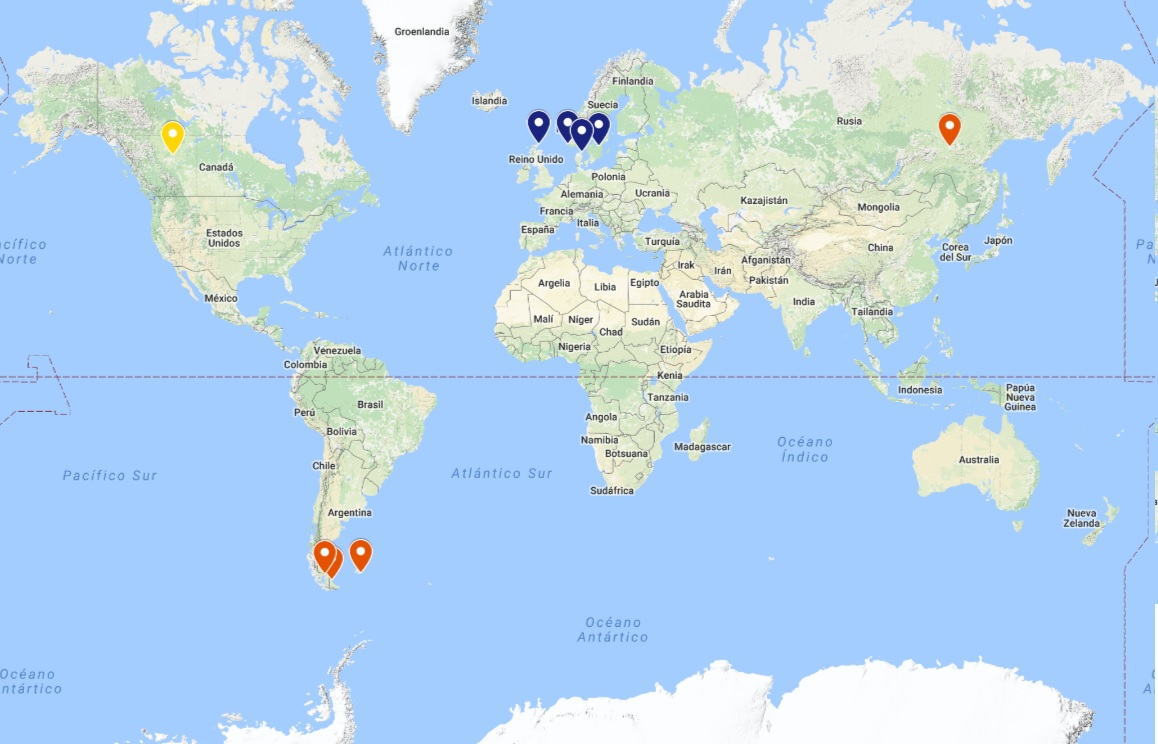
\includegraphics[scale=0.65]{Options.jpg}
\caption{Options for placing the 3 Ground Stations.}
\end{center}
\end{figure}
Given this possibilities a study of the legislation of the involved countries has to be done in order to know the viability of placing there the Ground Stations. The candidate countries, as is shown in the map, are: Canada, Argentina, Chile, Falkland Islands (Islas Malvinas), United Kingdom, Denmark, Norway, Sweden and Russia. 
